\documentclass{thesis/PatternRecognition}
\usepackage{thesis/scnu}
\usepackage{thesis/mynewcommand}
\usepackage{listings}
\usepackage{xcolor}
\usepackage{color}
\usepackage{multirow}
\usepackage{booktabs}
\usepackage{enumerate}
\usepackage{amsmath}

\graphicspath {{figures/}}%The folder containing pictures
\captionsetup{font={footnotesize}}
\definecolor{darkgreen}{rgb}{0,0.6,0}
\definecolor{underground}{rgb}{0.949,0.949,0.949}
\definecolor{strcolor}{rgb}{0.8,0,0.8}
\colorlet{stringcolour}{red!60!black}
\colorlet{keywordcolour}{magenta!90!black}
\colorlet{exceptioncolour}{yellow}
\colorlet{commandcolour}{blue!60!black}
\colorlet{numpycolour}{blue!60!green}
\colorlet{literatecolour}{magenta!90!black}
\colorlet{promptcolour}{green!50!black}
\colorlet{specmethodcolour}{violet}
\colorlet{commentcolour}{green!50!black}

%\numberwithin{eqnarray}{section}


\begin{document}

\lstset
{
language=python,
numbers=left,
numberstyle=\color{blue}, 						%代码编号
%stepnumber=0,									%代码编号步长
keywordstyle=\color{keywordcolour}\bfseries,			%关键字颜色
commentstyle=\color{commentcolour},					%注释颜色
%frame=shadowbox,								%边框
breaklines=true, 								%自动折行
stringstyle=\color{stringcolour},				%字符串颜色
backgroundcolor=\color{underground},			%背景色
xleftmargin=0cm,xrightmargin=0cm, aboveskip=1cm, %设置边距
basicstyle=\small,								%基本字体字号  
rulesepcolor=\color{red!20!green!20!blue!20},
flexiblecolumns=true, 
breakautoindent=true,
%python特有关键字
emph={and,break,class,continue,def,yield,del,elif ,else,%
except,exec,finally,for,from,global,if,import,in,%
lambda,not,or,pass,print,raise,return,try,while,assert,with},
emphstyle=\color{blue}\bfseries,
emph={[2]True, False, None},
emphstyle=[2]\color{keywordcolour},
emph={[3]object,type,isinstance,copy,deepcopy,zip,enumerate,reversed,list,len,dict,tuple,xrange,append,execfile,real,imag,reduce,str,repr},
emphstyle=[3]\color{commandcolour},
emph={Exception,NameError,IndexError,SyntaxError,TypeError,FileNotFoundError,ValueError,OverflowError,ZeroDivisionError},
emphstyle=\color{exceptioncolour}\bfseries ,
emph={[4]ode, fsolve, sqrt, exp, sin, cos,arctan, arctan2, arccos, pi,  array, norm, solve, dot, arange, , isscalar, max, sum, flatten, shape, reshape, find, any, all, abs, plot, linspace, legend, quad, polyval,polyfit, hstack, concatenate,vstack,column_stack,empty,zeros,ones,rand,vander,grid,pcolor,eig,eigs,eigvals,svd,qr,tan,det,logspace,roll,min,mean,cumsum,cumprod,diff,vectorize,lstsq,cla,eye,xlabel,ylabel,squeeze},
emphstyle=[4]\color{numpycolour},
emph={[7]range},
emphstyle={[7]\color{keywordcolour}\bfseries},
emph={[8]1, 2, 3, 4, 5, 6, 7, 8, 9, 0},
emphstyle={[8]\color{keywordcolour}\bfseries},
escapeinside=``
}



%		\ctitle{模式识别课程模板}
		\cauthorinfo{陈伟哲}{华南师范大学}{广州}{510631}{cosmo\_chan@126.com}
\cabstract{
本模板适用于模式识别课程, 当然根据要求稍加修改cls文件也能用于其他地方, 本文标题采用黑体三号, 作者采用仿宋四号, 作者信息采用宋体小五, 一级标题采用黑体小三, 二级标题采用黑体四号, 三级标题采用黑体小四, 正文采用5号ctexart默认字体.本模板使用xelatex编译(一些编辑器的默认编译模式是pdflatex,对中文的支持没xelatex好,请使用xelatex编译) 希望本模板能给你带来方便, 让你更加喜欢\LaTeX 的方便优雅.
如果参考文献部分编译给出警告提示,请再次编译.本文档会给出一些示例效果.
}

        \etitle{A Thesis for Data Mining Class}
        \eauthorinfo{Cosmo}{SCNU}{Guangzhou}{510631}{cosmo\_chan@126.com}
\eabstract{
Unfortunately, I have no time to translate the Chinese abstract, if you would like to make our thesis look better, feel free to contact me!
Unfortunately, I have no time to translate the Chinese abstract, if you would like to make our thesis look better, feel free to contact me!
Unfortunately, I have no time to translate the Chinese abstract, if you would like to make our thesis look better, feel free to contact me!
}

\newpage

\section{BP神经网络}
\subsection{神经网络的构造与前向传播}
神经网络是由单个或多个神经元组成。下面是单个神经元的构造。
\begin{center}
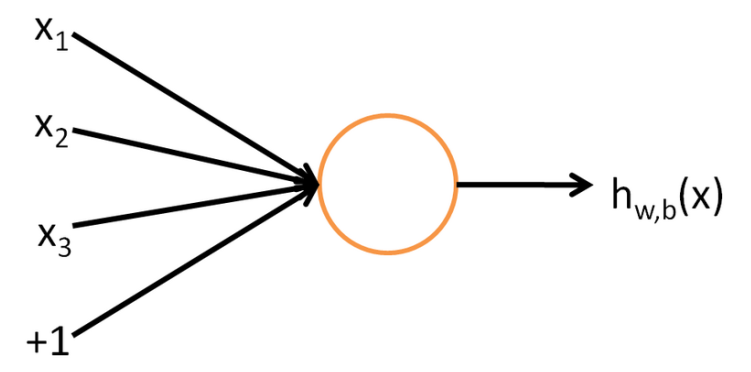
\includegraphics[scale=0.5]{../figures/NN1.png}\\
\textbf{图1}:神经元 
\end{center}
该神经元的输入由三个数据$x_1,x_2,x_3$以及偏置项(bias)+1组成,通过神经元后输出的表达式为
\begin{eqnarray}
h_{W,b}(x)=f(W^Tx+b)=f(\sum_{i=1}^3 W_ix_i+b)
\end{eqnarray}
其中$f$为激活函数。激活函数是为了将线性项$W^Tx$变换为非线性。在BP中,较常用的激活函数为sigmoid函数,其表达式如下
\begin{eqnarray}
f(z)=\frac{1}{1+\exp(-z)}
\end{eqnarray}
另外,令$b=w_0$,则可重新定义$W=(w_0,w_1,w_2,w_3)^T$,$x=(1,x_1,x_2,x_3)$,于是可将上式写为
\begin{eqnarray}
h_{W,b}(x)=f(W^Tx)
\end{eqnarray}
下面讨论神经网络。多个神经元可以组成一个层,多个层互相连接可以组成神经网络。其中,接受数据输入的层为输入层,数据计算后的数据的输出层,中间的层则称为隐含层。为下图是含有两个隐含层的神经网络。
\begin{center}
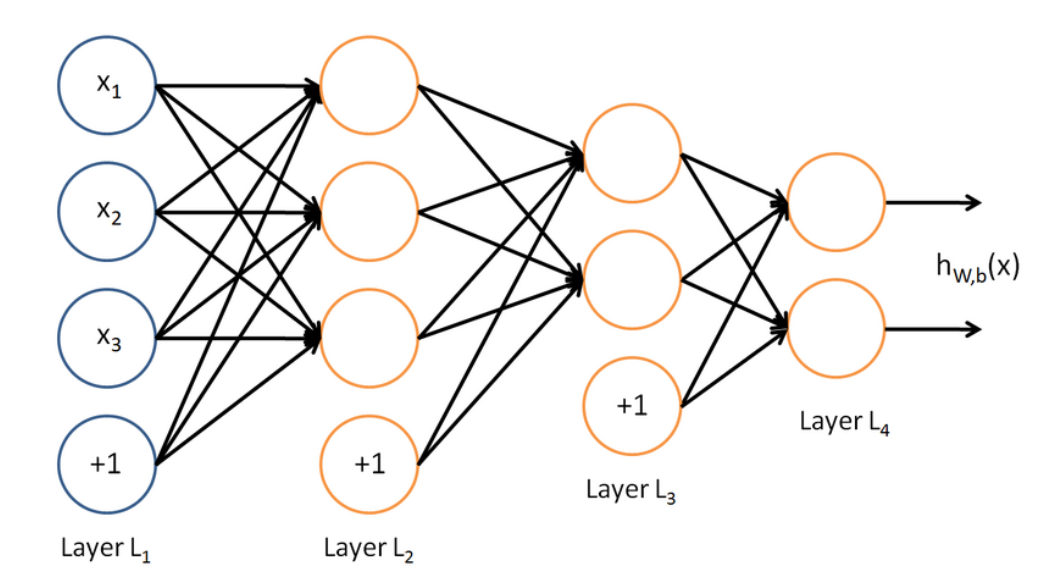
\includegraphics[scale=0.5]{../figures/NN2.png}\\
\textbf{图2}:含有两个隐含层的神经网络
\end{center}
如图,最左边的为输入层,即图中的Layer L1,最右边的为输出层,即图中的Layer L4,中间的所有层,即图中的Layer L2,Layer L3为隐含层。

我们用$n_l$来表示网络的层数,记第$i$层为$L_i$,于是输入层为$L_1$,输出层为$L_{n_l}$。由于神经网络可以有任意多的隐层以及隐藏神经元,则我们记$\samplet{W}{l}{ij}$为第$l$层第$j$单元以及第$l+1$层第$i$单元之间的连接权重,$\samplet{b}{l}{i	}$为第$L+1$层第$i$单元的偏执。我们用$\samplet{a}{l}{i}$表示第$l$层第$i$单元的激活值(输出值),则有
\begin{eqnarray}
\samplet{a}{l+1}{i}=f(\sum_{j=1}^{S_l}\samplet{W}{l}{ij}\samplet{a}{l}{j}+\samplet{b}{l}{i})
\end{eqnarray}
其中当$l=1$时,$\sample{a}{l}=x$,$x$为输入向量$(x_1,x_2,\cdots,x_{S_l})$,$S_l$指第$l$层的神经元个数,我们用$\samplet{z}{l+1}{i}$表示第$l+1$层第$i$单元输入加权和(包括偏置),即
\begin{eqnarray}
\samplet{z}{l+1}{i}=\sum_{j=1}^{S_t}\samplet{W}{l}{ij}\samplet{a}{l}{j}+\samplet{b}{l}{i}
\end{eqnarray}
则有
\begin{eqnarray}
\samplet{a}{l+1}{i}&=&f(\samplet{z}{l+1}{i})\\
h_{W,b}(x)&=&\sample{a}{n_l}=f(\sample{z}{n_l})
\end{eqnarray}
上述过程称为神经网络的前向传播。
\subsection{神经网络的反向传播}
根据上面的前向传播,我们设神经网络的各层表示为$L_1,L_2,\cdots,L_{n_l}$,其中,$L_{n_l}$为输出层,对于输出层,假设输出层输出为$t=\sample{a}{n_l}$,$y$为标签,则若为回归问题,则代价函数使用MSE,即
\begin{eqnarray}
J(W,b;x,y)=\frac{1}{2}||t-y||^2
\end{eqnarray}
接下来计算输出层的残差
\begin{eqnarray}
\begin{aligned}
\samplet{\delta}{n_l}{i}&=\frac{\partial}{\partial \samplet{z}{n_l}{i}}J(W,b;x,y)\\
&=\frac{\partial}{\partial \samplet{z}{n_l}{i}}\frac{1}{2}||y-h_{W,b}(x)||^2\\
&=\frac{\partial}{\partial \samplet{z}{n_l}{i}}\frac{1}{2}\sum_{j=1}^S{_{n_l}}(y_i-\samplet{a}{n_l}{j})^2\\
&=\frac{\partial}{\partial \samplet{z}{n_l}{i}}\frac{1}{2}\sum_{j=1}^S{_{n_l}}(y_i-f(\samplet{z}{n_l}{i}))^2\\
&=-(y_i-f(\samplet{z}{n_l}{i}))\cdot f'(\samplet{z}{n_l}{i})\\
&=-(y_i-\samplet{a}{n_l}{i})\cdot f'(\samplet{z}{n_l}{i})
\end{aligned}
\end{eqnarray}
下面考虑残差的递推算法,以输出层前一层为例。由前向传播我们可以推导出
\begin{eqnarray}
\samplet{z}{l+1}{i}=\sum_{j=1}^{S_l}\samplet{W}{l}{ij}f(\samplet{z}{l}{i})+\samplet{b}{l}{i}
\end{eqnarray}
则有
\begin{eqnarray}
\samplet{z}{n_i}{i}=\sum_{j=1}^{S_l} \samplet{W}{n_l-1}{ij}f(\samplet{z}{n_l-1}{i})+\samplet{b}{n_l-1}{i}
\end{eqnarray}
于是有
\begin{eqnarray}
\frac{\partial \samplet{z}{n_l}{i}}{\partial \samplet{z}{n_l-1}{i}}=\sum_{j=1}^{S_l}\samplet{W}{n_l-1}{ij}f'(\samplet{z}{n_l-1}{i})
\end{eqnarray}
则可以得到输出层前一层的残差
\begin{eqnarray}
\begin{aligned}
\samplet{\delta}{n_l-1}{i} &= \frac{\partial}{\partial \samplet{z}{n_l-1}{i}}J(W,b;x,y)\\
&= \frac{\partial J(W,b;x,y)}{\partial \samplet{z}{n_l}{i}}\cdot\frac{\partial \samplet{z}{n_l}{i}}{\partial \samplet{z}{n_l-1}{i}}\\
&= \sum_{j=1}^{S_l}\samplet{\delta}{n_l}{j}\samplet{W}{n_l-1}{ij}f'(\samplet{z}{n_l-1}{i})
\end{aligned}
\end{eqnarray}
将$n_l-1$与$n_l$的关系替换为$l$与$l+1$的关系,则可得到
\begin{eqnarray}
\samplet{\delta}{l}{i}=\frac{\partial}{\partial \samplet{z}{l}{i}}J(W,b;x,y)=
\left(
	\begin{aligned}
		\sum_{j=1}^{S_{l+1}}\samplet{W}{l}{ji}\samplet{\delta}{l+1}{j}
	\end{aligned}
\right)
f'(\samplet{z}{l}{i})
\end{eqnarray}
若取函数$f$为sigmoid函数,则有
\begin{eqnarray}
f'(\samplet{z}{l}{i})=f(\samplet{z}{l}{i})\circ(1-f(\samplet{z}{l}{i}))=\samplet{a}{l}{i}\circ(1-\samplet{a}{l}{i})
\end{eqnarray}
其中$\circ$代表点乘。于是可得到$\samplet{\sigma}{l+1}{j}$到$\samplet{\sigma}{l}{j}$的递推式:
\begin{eqnarray}
\samplet{\delta}{l}{i}=
\left(
	\begin{aligned}
		\sum_{j=1}^{S_{l+1}}\samplet{W}{l}{ji}\samplet{\delta}{l+1}{j}
	\end{aligned}
\right)
(\samplet{a}{l}{i}\circ(1-\samplet{a}{l}{i}))
\end{eqnarray}
反向传播,一般采用梯度下降法对每一层的权重进行调整,即
\begin{eqnarray}
\samplet{W}{l}{ij}=\samplet{W}{l}{ij}-\alpha\frac{\partial}{\partial \samplet{W}{l}{ij}}J(W,b;x,y)
\end{eqnarray}
其中,$\alpha$是学习率。因而需要求权重$\samplet{W}{l}{ij}$对于代价函数的偏导,此时可使用当前层的残差来进行计算,即
\begin{eqnarray}
\frac{\partial}{\partial \samplet{W}{l}{ij}}J(W,b;x,y)=\frac{\partial J(W,b;x,y)}{\partial \samplet{z}{l+1}{i}}\frac{\samplet{z}{l+1}{i}}{\samplet{W}{l}{ij}}
\end{eqnarray}
又有
\begin{eqnarray}
\frac{\samplet{z}{l+1}{i}}{\samplet{W}{l}{ij}}=\frac{\left( \sum_{j=1}^{S_l}\samplet{W}{l}{ij}f(\samplet{z}{l}{i}) \right)}{\samplet{W}{l}{ij}}=f(\samplet{z}{l}{i})=\samplet{a}{l}{i}
\end{eqnarray}
于是可得
\begin{eqnarray}
\frac{\partial}{\partial \samplet{W}{l}{ij}}J(W,b;x,y)=\samplet{a}{l}{j}\samplet{\delta}{l+1}{i}
\end{eqnarray}
综上,可以总结BP神经网络算法
\paragraph{BP神经网络算法}
\begin{lstlisting}[language=python]
`输入:训练输入$x$,训练输出$y$,学习率$\alpha$`
while `未达到收敛条件`
    `
	输入训练输入,训练输出,学习率\\
	1.初始化神经网络的权重与偏置\\
	2.对输入进行前向传播,得到除输入层外每一层($L_2,\cdots,L_{n_l}$)的激活值$\sample{a}{2},\cdots,\sample{a}{n_l}$\\
	3.计算各层残差:\\
	(1)对输出层(第$n_l$层)
	\begin{eqnarray}
	\sample{\delta}{n_l}=-(y-\sample{a}{n_l})\cdot(\sample{a}{l}\circ(1-\sample{a}{l}))
	\end{eqnarray}
	(2)对于$l=n_l-1,\cdots,2$各层,可递推得出残差值
	\begin{eqnarray}
	\sample{\delta}{l}=((\sample{W}{l})^T\sample{\delta}{l+1})\cdot(\sample{a}{l})
	\end{eqnarray}
	(3)计算损失函数对每一层权重的偏导数值
	\begin{eqnarray}
	\nabla_{\sample{W}{l}}J(W,b;x,y)=\sample{\delta}{l+1}(\sample{a}{l})^T
	\end{eqnarray}
	(4)更新参数
	\begin{eqnarray}
	\sample{W}{l}=\sample{W}{l}-\alpha\nabla_{\sample{W}{l}}J(W,b;x,y)
	\end{eqnarray}
    `
end

\end{lstlisting}

若为多分类问题,先对$y$进行one-hot处理得到$p$维向量$(y_1,y_2,\cdots,y_p)$(假设$y$有$p$种取值),并将输出层的激活函数选为softmax,即
\begin{eqnarray}
\samplet{a}{n_l}{i}=f_s(\samplet{z}{n_l}{i})=\frac{e^{\samplet{z}{n_l}{i}}}{\sum_je^{\samplet{z}{n_l}{j}}}
\end{eqnarray}
并且代价函数使用交叉熵损失函数
\begin{eqnarray}
J(W,b;x,y)=-\sum_i y_i\log \samplet{a}{n_l}{i}
\end{eqnarray}
则输出层残差为
\begin{eqnarray}
\begin{aligned}
\samplet{\delta}{n_l}{i}&= \frac{\partial J}{\partial \samplet{z}{n_l}{i}}\\
&=\sum_i\frac{\partial J}{\samplet{a}{n_l}{i}}\cdot\frac{\partial \samplet{a}{n_l}{i}}{\partial \samplet{z}{n_l}{i}}\\
&=\sum_i\frac{\partial -\sum_i y_i\log\samplet{a}{n_l}{i}}{\samplet{a}{n_l}{i}}\cdot\frac{\partial \samplet{a}{n_l}{i}}{\partial \samplet{z}{n_l}{i}}\\
&=-\sum_i\frac{y_i}{\samplet{a}{n_l}{i}}\frac{\partial \samplet{a}{n_l}{i}}{\partial \samplet{z}{n_l}{j}}
\end{aligned}
\end{eqnarray}
当$i=j$时,记$e^{\samplet{z}{n_l}{j}}=e^A$,$\sum_{k\neq j}e^{\samplet{z}{n_l}{k}}=e^B$,显然有$e^A+e^B=\sum_ie^{\samplet{z}{n_l}{i}}$,于是
\begin{eqnarray}
\begin{aligned}
\frac{\partial \samplet{a}{n_l}{i}}{\partial \samplet{z}{n_l}{j}} &= \frac{\partial \samplet{a}{n_l}{j}}{\partial \samplet{z}{n_l}{j}}\\
&= \frac{\partial \frac{e^A}{e^A+e^B}}{\partial A}\\
&= \frac{e^A(e^B+e^A)-e^{2A}}{(e^A+e^B)^2}\\
&= \frac{e^Ae^B}{(e^A+e^B)^2}\\
&= \frac{e^A}{e^A+e^B}\frac{e^B}{e^A+e^B}\\
&= \frac{e^A}{e^A+e^B}(1-\frac{e^A}{e^A+e^B})\\
&= \samplet{a}{n_l}{j}(1-\samplet{a}{n_l}{j})
\end{aligned}
\end{eqnarray}
\subsection{激活函数}
\paragraph{sigmoid}
sigmoid函数表达式如下
\begin{eqnarray}
f(x)=\frac{1}{1+e^{-x}}
\end{eqnarray}
其图像如下图所示
\begin{center}
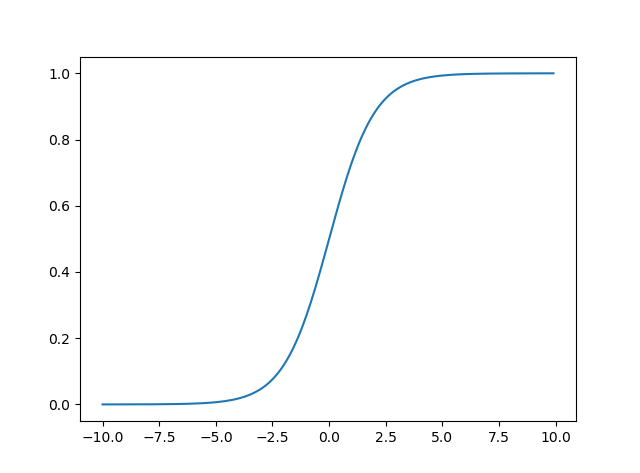
\includegraphics[scale=0.5]{../figures/NN3.png} 
\end{center}
sigmoid激活函数考虑将输入值映射到$(0,1)$的区间中,该函数在定义域内连续,且导数大于0。它也有较为简单的求导结果
\begin{eqnarray}
f'(x)=f(x)(1-f(x))
\end{eqnarray}
但是在神经网络中,特别是对于层数较多的网络,通常不采用sigmoid作为激活函数,主要是因为其容易产生梯度消失的情况。当输入非常大或非常小的时候,其梯度趋近于0,反向传播的过程中直接导致梯度无法传播,无法有效地调整权重。虽然做标准化可以让数据近似服从正态分布,但梯度消失仍有可能产生,在学习过程中可能会产生输入较大或较小的情况。或许这个问题可以用batch-normalization来缓解,但明显采取一种更佳的激活函数是较为可取的做法。
\paragraph{ReLU}
ReLU函数表达式如下
\begin{eqnarray}
f(x)=\max\{0,x\}
\end{eqnarray}
图像如下
\begin{center}
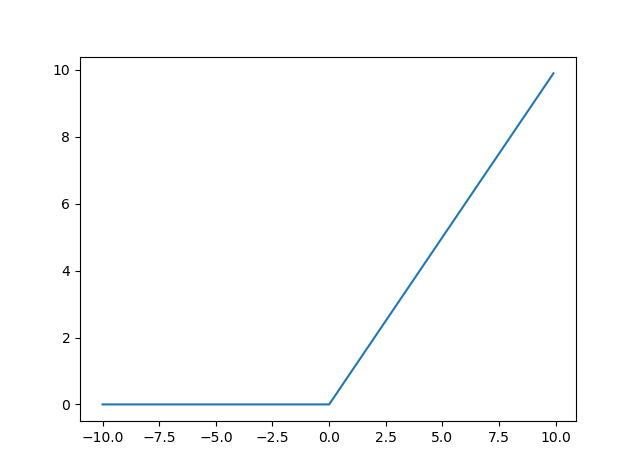
\includegraphics[scale=0.5]{../figures/NN5.png} 
\end{center}
其决定它有非常简单的求导结果
\begin{eqnarray}
f'(x)=
\left\lbrace
\begin{aligned}
1,\ x>0\\
0,\ x<0
\end{aligned}
\right.
\end{eqnarray}
RuLU收敛能比sigmoid快的多,一方面其计算快,比起sigmoid函数的导数需要指数运算,RuLU只需要做大小的比较。另一方面,其梯度经过多个层传播之后,多数能够保持原汁原味,比起sigmoid会梯度消失要好得多。然而,RuLU也有弱点,当$x<0$时$f(x)$为0,梯度为0,这直接导致该神经元失活。因而在训练过程中,要注意取较小的学习率。
\paragraph{Leaky ReLU}
Leaky ReLU是针对RuLU的弱点而改进的,其考虑用一个比较小的数去替代$x<0$时的$f(x)=0$,即
\begin{eqnarray}
f'(x)=
\left\lbrace
\begin{aligned}
x,\ x>0\\
ax,\ x<0
\end{aligned}
\right.
\end{eqnarray}
图像如下
\begin{center}
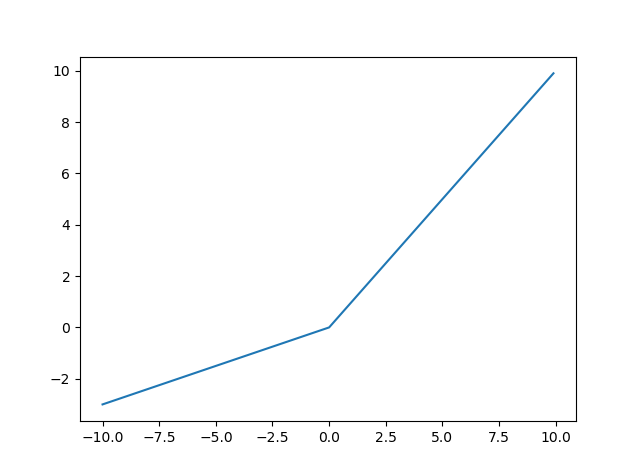
\includegraphics[scale=0.5]{../figures/NN7.png} 
\end{center}
其求导结果为
\begin{eqnarray}
f'(x)=
\left\lbrace
\begin{aligned}
1,\ x>0\\
a,\ x<0
\end{aligned}
\right.
\end{eqnarray}
这个方法可以使$x<0$处避免失活,但是额外引入了超参数$a$。
\paragraph{PReLU}PReLU是针对Leaky ReLU的进一步优化,其考虑在反向传播过程中,也对$a$进行学习,从而避免引入超参数$a$。一些实验$\ ^{[1]}$证明这种优化能取到好的学习效果。
\subsection{传统BP网络的应用}
以上介绍的BP网络的算法以及较为传统的结构,我们想探究随着图像尺寸的变化(即输入大小)以及隐含层神经元。首先我们制备数据,通过opencv的方法,将输入图像归一化为同一大小,分别为$64\times 64$,$96\times 96$,$128\times 128$,学习率设置0.03,优化函数采用Mini-batch,以8个样本作为一个batch,epoch设为600。首先考虑当隐含层分别设为1000和500时,图像大小为$64\times 64$时,模型的训练准确率如下:
\begin{center}
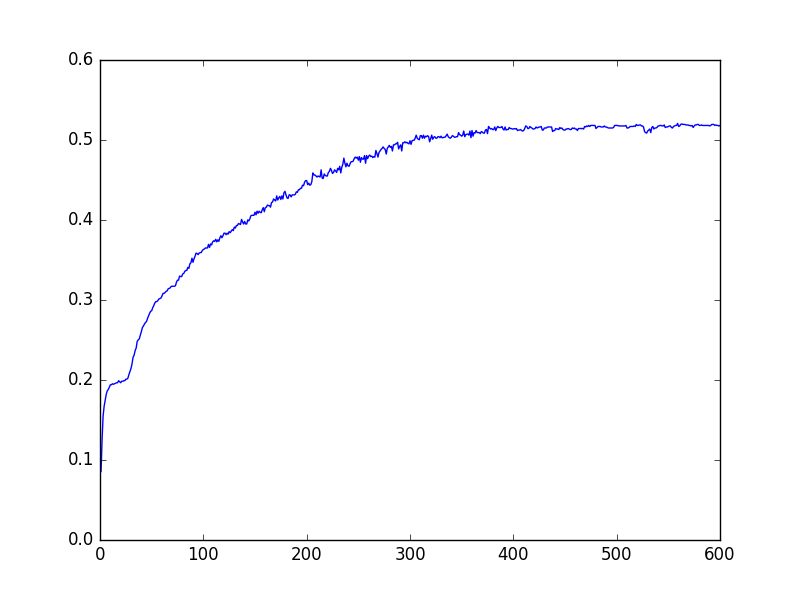
\includegraphics[scale=0.5]{../figures/Log/BP_new1/BP_new1_acc.png} 
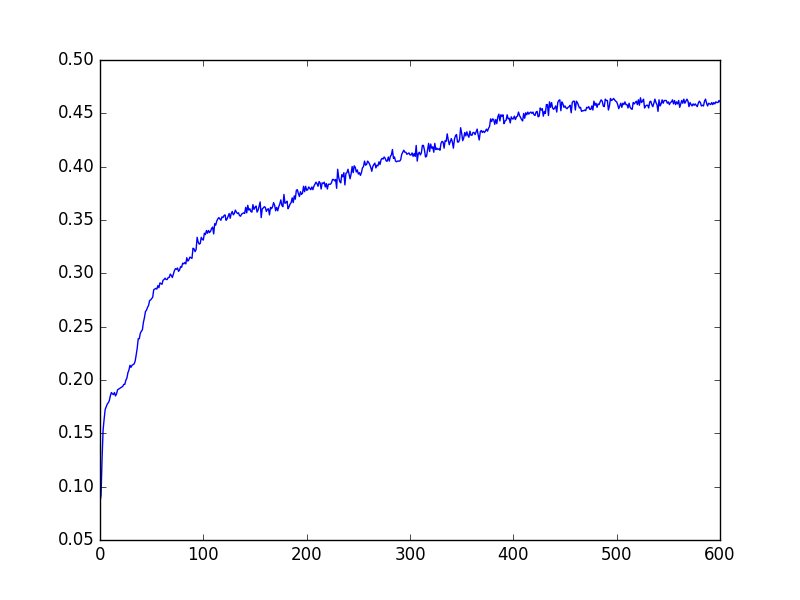
\includegraphics[scale=0.5]{../figures/Log/BP_new4/BP_new4_acc.png} \\
图像大小为$64\times 64$时,隐含层为1000和500的准确率图
\end{center}
从图中可以看出,隐含层为1000时比500好接近5\%,收敛速度上,前者在epoch为300时就趋于稳定,后者在epoch为450时趋于稳定。其原因四隐含层1000时,其自由度比500大,随着参数的增加,更有可能得到偏差小的模型。从实验可以看出,前者相比于后者在达到较低偏差的同时,其方差也不会很大。

当隐含层分别设为1000和500时,图像大小为$96\times 96$时,模型的训练准确率如下:
\begin{center}
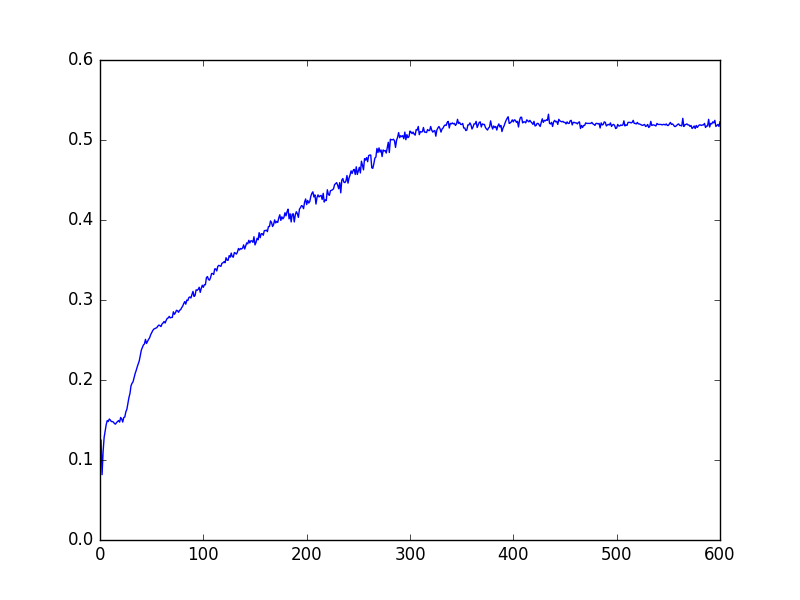
\includegraphics[scale=0.5]{../figures/Log/BP_new2/BP_new2_acc.png} 
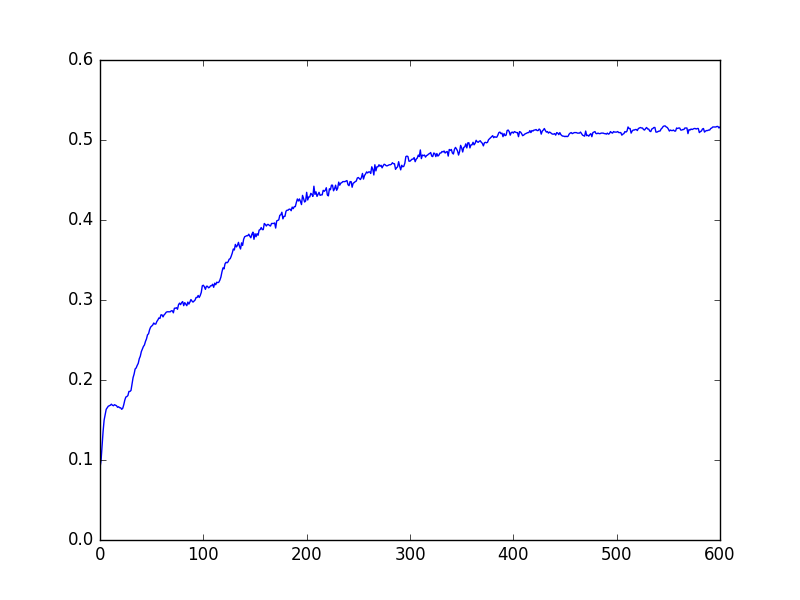
\includegraphics[scale=0.5]{../figures/Log/BP_new5/BP_new5_acc.png} \\
图像大小为$96\times 96$时,隐含层为1000和500的准确率图
\end{center}
从图中可以看出,隐含层1000与500在准确率上持平,为50\%左右。由于随着图像的尺寸增加,过拟合的风险增大。而前者相比于后者有更低的模型复杂度,一定程度上抵制了过拟合。而过拟合的风险随着图像尺寸的增大而增大的现象,我们将在下图进一步看到:

当隐含层分别设为1000和500时,图像大小为$128\times 128$时,模型的训练准确率如下:
\begin{center}
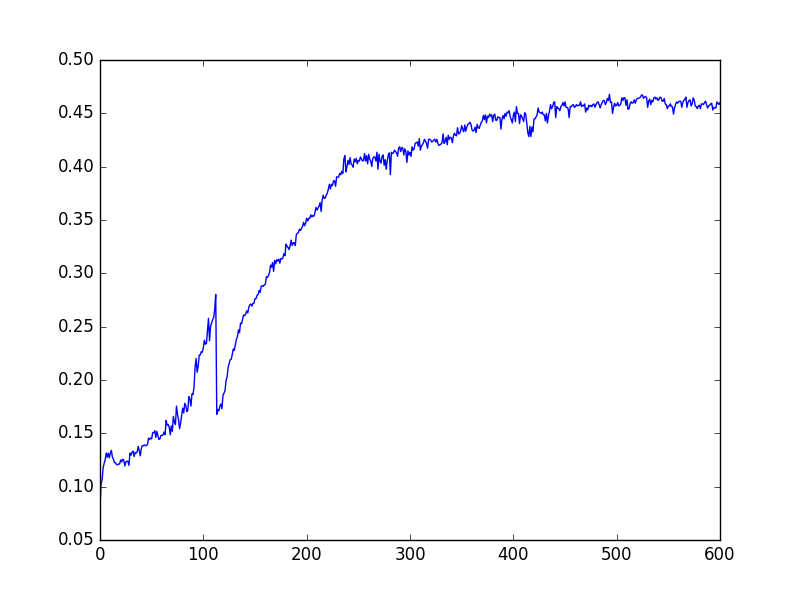
\includegraphics[scale=0.5]{../figures/Log/BP_new3/BP_new3_acc.png} 
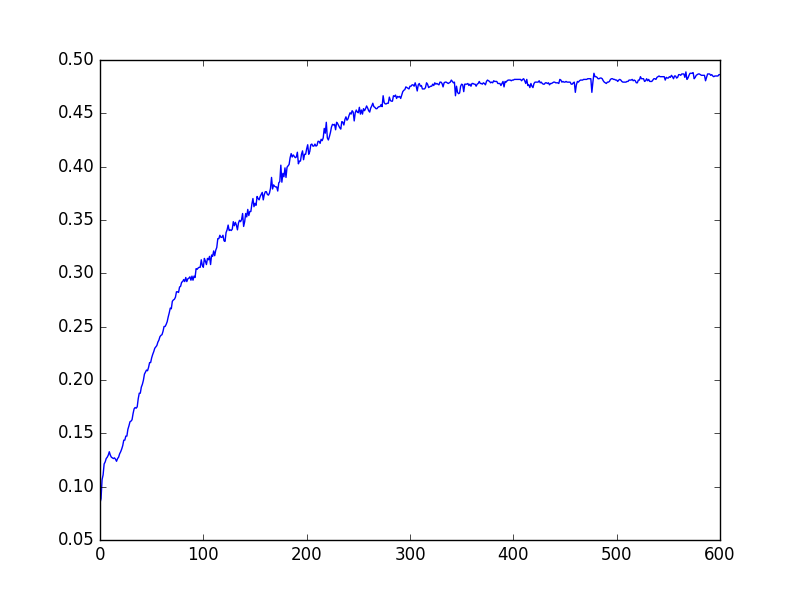
\includegraphics[scale=0.5]{../figures/Log/BP_new6/BP_new6_acc.png} \\
图像大小为$128\times 128$时,隐含层为1000和500的准确率图
\end{center}
从图中可看出,当隐含层为1000时,其训练过程中准确率出现了大幅度的震荡,而且准确率收敛在了45\%左右,而隐含层为500的模型相比隐含层为1000的模型的更加健壮,而且准确率接近50\%,比隐含层为1000的模型高了大概4\%。

综上,我们可以得到各个模型的准确率表格
\begin{center}
\begin{tabular}{cccc}
\toprule[2pt]
\  & $64\times 64$ & $96\times 96$ & $128\times 128$ \\ 
\midrule[1pt]
1000 & 0.518188 & \textbf{0.522655} & 0.460115 \\ 
500 & 0.460753 & 0.516273 & 0.48628 \\ 
\bottomrule[2pt]
\end{tabular} 
\end{center}
可以看出,在保证图像不要过大而导致过拟合下,隐含层1000的模型比隐含层500的模型性能更优。

\subsection{梯度下降方法}
梯度下降法的选取能影响收敛速度与质量,	它也是模型构成的一部分。在应用中一般有如下的梯度下降法可供选择
\paragraph{批量梯度下降法}
批量梯度下降法(Batch Gradient Descent )考虑在计算了所有样本之后再对参数进行更新,即
\begin{eqnarray}
\sample{W}{l}=\sum_{i=1}^m\sample{W}{l}-\alpha\nabla_{\sample{W}{l}}J(W,b;\sample{x}{i},\sample{y}{i})
\end{eqnarray} 
由于通常训练的样本非常大,若在计算所有样本之后再进行参数更新,会让更新的速度减慢。另外,模型实现一般会采用矩阵运算,BGD占的内存会非常多,从而影响计算速度。
\paragraph{随机梯度下降法}
随机梯度下降法(Stochastic Gradient Descent )的想法与BGD截然不同,计算每一个样本之后便进行一次反向传播,对参数进行更新,即
\begin{eqnarray}
\sample{W}{l}=\sample{W}{l}-\alpha\nabla_{\sample{W}{l}}J(W,b;x,y)
\end{eqnarray}
相比之下,SGD的训练速度比BGD快得多,在BGD进行一次反向传播的时间内,SGD已经进行过多次传播。但是在梯度下降过程中,SGD容易出现震荡,由于单个样本并不能代表梯度最大的方向,也有可能导致解非最优的情况。
\paragraph{小批量梯度下降法}
小批量梯度下降法(Mini-batch Gradient Descent )考虑了批量梯度下降法和随机梯度下降法的优缺点,并进行结合,考虑将数据集划分成多个含有较小数据的batch,然后对这些batch分别采用BGD。下面给出第$i$个batch的训练公式
\begin{eqnarray}
\sample{W}{l}=\sum_{(x,y)\in b_i}^m\sample{W}{l}-\alpha\nabla_{\sample{W}{l}}J(W,b;x,y)
\end{eqnarray}
其中,$b_i$代表当前batch所包含的训练样本$(x,y)$的集合。
\paragraph{动量梯度下降法}
无论是SGD还是MGD,即便MGD已在SGD上做了优化,在训练过程中仍可能会有振荡的风险。一种优化的方法是基于SGD,在对参数$\sample{W}{l}$进行更新时,会考虑上一次的更新幅度,若是当前的梯度方向与上一次的相同,则能够加速收敛,反之则能抑制更新,这也是采用了动量的想法。其算法如下
\begin{lstlisting}[language=python]
`输入:学习率$\epsilon$,动量参数$\alpha$`
`$t_{dW} = \alpha t_{dW} + (1-\alpha) t_{dW}$`
`$W = W - \epsilon t_{dW}$`
\end{lstlisting}
\subsection{正则化与dropout}
机器学习中,常会发生过拟合的情况,通常引起这种情况的原因有数据量过小、维度过大、模型复杂度过大等,而此现象是方差过大且偏差太小所致。通常维度过大可采用特征选择的方法来降维,而模型复杂度可以用正则化项来限制。它是考虑在损失函数中添加能反映出模型复杂度的项。例如在神经网络中,下面的损失函数的第二项称为L2正则化
\begin{eqnarray}
J(W,b;x,y) = -\sum_i y_i \log \samplet{a}{n_l}{i} + \lambda\sum_w w^2
\end{eqnarray}
我们可以把损失函数看出是由偏差衡量项(第一项)和方差衡量项(第二项)组成,其本质是偏差、方差权衡,权衡通过$\lambda$来实现。

除了L2正则化之外,常用的还有L1正则化,为如下形式
\begin{eqnarray}
J(W,b;x,y) = -\sum_i y_i \log \samplet{a}{n_l}{i} + \lambda\sum_w |w|
\end{eqnarray}

神经网络中,除了加入正则化项之外,还能考虑在每次训练中,让所有神经元以一定概率失活,即封闭该神经元的输出,此方法成为dropout。因而在每次训练中,网络结构都不一样,在降低模型复杂度的同时,也是对于多个模型的集成,其示意图如下。
\begin{center}
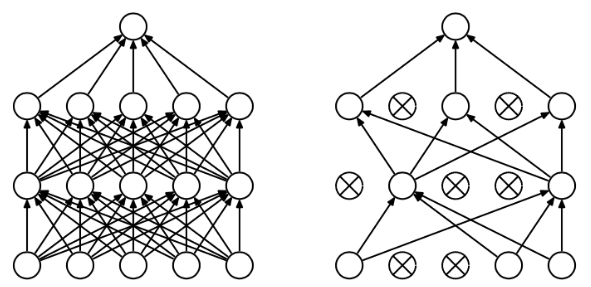
\includegraphics[scale=0.5]{../figures/dropout.png} \\
dropout工作原理示意图
\end{center}
\subsection{BP神经网络+}

\section{卷积神经网络}
\subsection{卷积神经网络概述}
卷积神经网络的特点在于能够提取出一个图像中的各种特征。其原理为自然图像的一
部分的统计特性与其他部分是一样的。也就是说在这一部分学习的特征也能用在另一部分
上,所以对于这个图像上的所有位置,我们都能使用同样的学习特征(权值)。
我们提取一种特征用一种卷积核,卷积核为下图左边图像黄色部分,卷积核的权值为
黄色部分右下红色字体。
\begin{center}
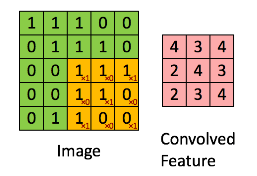
\includegraphics[scale=0.7]{../figures/conv.png} 
\end{center}
设大矩阵的大小为为$d\times d$,利用大小为$m\times m$的卷积核可以得到特征提取
降维后的大小为$(d-m+1)\times(d-m+1)$的矩阵。这个过程为一个特征的提取。在卷积
的过程中,从原图像(Image)矩阵$I$生成的卷积特征矩阵$C$(Convolved Feature)中的
每个元素为:
\begin{eqnarray}
C_{ij}=\sum_{u=1}^m\sum_{v=1}^mw_{uv}I_{i+u-1,j+v-1}
\end{eqnarray}
其中,$i,j\in(d-m+1)$
对于卷积特征矩阵(Convolved feature)我们下一步进行池化。池化的目的是对图像
不同位置进行聚合统计来描述大的图像。聚合统计可以通过计算一个区域上某个特定特征
的平均值或者最大值,这样可以降低更多的维度以及不容易过拟合。如果选择图像中连续
的范围作为池化区域,并且只是池化重复的隐藏单元产生的特征,那么这些池化单元具有
平移不变性。这就意味着即使图像经历了一个小的平移之后依然会产生相同的池化特征。
池化过程如下图:
\begin{center}
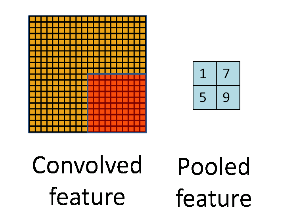
\includegraphics[scale=0.7]{../figures/pool.png} 
\end{center}
我们叫上图左图红色部分为一个池,并且通常取能够将卷积特征矩阵平均划分的大小的池。
池化后我们得到池化特征矩阵$P$(Pooled feature),我们设卷积特征图像为长宽都为$c$的
矩阵,则池长宽设为$p$,若为最大池化则$P$的元素为:
\begin{equation}
P_{ij}=\max_{u\in[1,p],v\in[1,p]}\{C_{u+(i-1)\times(p+1),v+(j-1)\times(p+1)}\}
\end{equation}
其中,$i,j\in[1,\frac{c}{p}]$。
若采用平均池化,则$P$的元素为
\begin{eqnarray}
P_{ij}=\frac{1}{p^2}\sum_{v=1}^p\sum_{u=1}^pC_{u+(i-1)\times(p+1),v+(j-1)\times(p+1)}
\end{eqnarray}
其中,$i,j\in[1,\frac{c}{p}]$。事实上,在设置卷积核时,一般将其设置为四维,各个维度分别为:卷积核长、卷积核宽、上一层的图像深度,卷积核个数。另外,对于一些深度学习的任务,是需要重复卷积很多次,为了实现这一目的,需要确保卷积之后图像长宽不变,于是在卷积之前通常在图像周围补足够个数的0,以扩大图像的尺寸,使得卷积之后的图像与原来的图像尺寸相同。

卷积神经网络其实可以包含两个大的部分,分别为特征提取层与分类器层。特征提取层包含若干个卷积层和池化层。在特征提取层中,只需要训练卷积层,而卷积层的共享参数与卷积核的属性,相比于全连接神经网络,参数更少,且抓住了图像的特征。特征提取层的输出需要转化之后,才能接入分类器层,一般的做法是将输出拉长为向量,而分类器层一般是用全连接的神经网络,最后接入softmax层,与标签计算损失函数,进而反向传播。下图是一种卷积网络结构,其对应的任务是手写数字识别。

\begin{center}
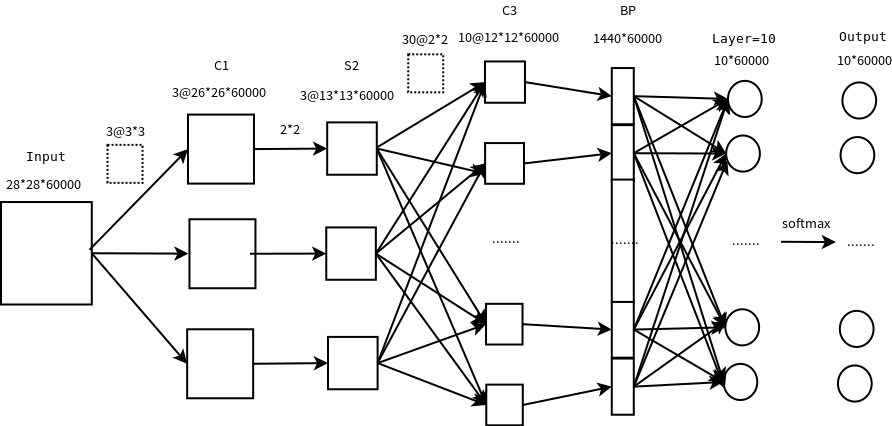
\includegraphics[scale=0.4]{../figures/CNN1.png} 
\end{center}
\subsection{经典CNN模型}
\paragraph{AlexNet}AlexNet结构上由8层隐含层组成,前五层为特征提取层,后三层为分类器层,用于做图像分类。其具体的结构如下:
\begin{center}
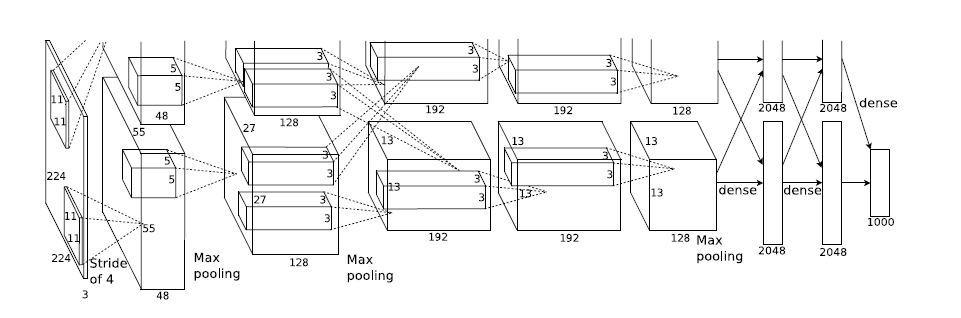
\includegraphics[scale=0.6]{../figures/AlexNet.png} \\
AlexNet结构,需注意的是,隐含层计算时分为上下部分计算,实际上是一个分布式计算的想法。
\end{center}
AlexNet当年提出来用已解决ImageNet的分类问题,对于$224\times224$像素的三通道照片,第一层使用$11\times11\times3\times96$的卷积核;第二层使用$5\times5\times96\times256$的卷积核,并进行最大池化;第三层使用$3\times3\times256\times384$的卷积核;第四层使用$3\times3\times384\times384$的卷积核;第五层使用$3\times3\times384\times256$的卷积核;之后连接全连接层,第六、七层都为4096个神经元,第八层则使用softmax。AlexNet的创新点在于激活函数采用了ReLU与dropout。
\paragraph{VGGNets}
\subsection{迁移学习}
\subsection{CNN+}



\subsection{Batch Normalization}



\section{RCNN}
\subsection{神经网络}
\subsection{卷积神经网络}
\subsubsection{AlexNet}
\subsubsection{VGGNet}
\subsection{Inception}
\subsection{ResNet}

\subsection{迁移学习}
\subsection{交并比}
交并比(Intersection-over-Union,Iou)是用于衡量候选框(candidate bound)与标记框(ground truth bound)相似程度的指标,其是两者的交叠率。假设候选框区域为$C$,标记框区域为$G$,则定义交并比$IoU$为
\begin{eqnarray}
IoU=\frac{C\cap G}{C\cup G}
\end{eqnarray}
%如图所示
若$IoU$越接近与1,说明重叠程度越大,效果越好。
\subsection{非极大值抑制}
非极大值抑制算法(Non-maximum suppression,NMS)本质为搜索局部的极大值,并抑制附近非极大值的元素。

若给定一个$n$个元素的一维数组$A$,该数组的顺序已定义了该数组的序。并定义领域$\epsilon$,对于某个元素$A[i]$,若$A[i]>A[j],j\in[i-\epsilon,i]$且$A[i]<A[j],j\in[i,i+\epsilon]$,则$A[i]$为极大值,否则,跳出$\epsilon$范围并重复上述操作,直到数组遍历完毕。其算法伪代码如下,其中,设$\epsilon=2$
\begin{lstlisting}[language=python]
Input: A
Output: MaximumSet
i=2
while i<=n-1
    if A[i]>A[i-1]
    	if A[i]>A[i+1]
            MaximumSet = MaximumSet `$\cup$` A[i]
    else
    	i=i+1
    	while i<=n-1 and A[i]<=A[i+1]
    		i=i+1
    	if i<=n-1
    		MaximumSet = MaximumSet `$\cup$` A[i]
    i=i+2
\end{lstlisting}

在物体检测中,由于初始化的候选边框数量很大,对于要检测的物体,其对应的边框很多,且边框之间的交叉重复特别严重,因此考虑用非极大值抑制来找到最佳的边框。

\subsection{选择性搜索}

\subsection{候选区域变换}
由于使用选择性搜索算法所产生的候选区域是长方形的,但其所包含的元素不定。又因为需要使用卷积神经网络对这些候选区域进行特征提取与降维,这就意味着需要将不定大小的候选区域变换为一个长宽(假设是$a\times b$)固定的区域。常见的方法如下
\paragraph{tightest square with context}该方法考虑的,首先是采用各向同性的方法,将候选区域扩展为$\max\{a,b\}\times\max\{a,b\}$的正方形区域。对于候选区域扩展后无法涉及的区域,用原来的图像对应的像素进行填补,之后再对该正方形进行裁剪,裁剪为$a\times b$。该想法可理解为扩展后加入背景。
\paragraph{tightest square without context}该方法是 tightest square with context的变体,其在候选区域扩展后无法涉及的区域的处理方法有所不同。其考虑的是对这部分区域不做处理。
\paragraph{warp}该方法采用的是各项异性的方法,直接把原来的图像,从长宽方向使用各自的比例进行放缩,直接放缩为$a\times b$ 。

%\pagestyle{fancy}
\rhead{}
\chead{Machine Learning Note}
\lhead{}
\cfoot{}
\rfoot{\thepage}



%\tableofcontents       %输出目录
%\newpage
%if you like to use bibtex, you can delete the above line and use the following two lines

%\bibliographystyle{plain}
%\bibliography{YourFile/reference}
\end{document}
